\documentclass[a0,portrait]{a0poster}

%%%%%%%%%%%%%%%%%%%%%%%%%%%%%%%%%%%%%%%%%%%%%%%%%%%%%%%%%%%%%
\usepackage[utf8]{inputenc}
\usepackage{multicol}
\usepackage[svgnames]{xcolor}
\usepackage{times}
\usepackage{dsfont}
\usepackage{graphicx}
\usepackage{booktabs}
\usepackage[font=small,labelfont=bf]{caption}
\usepackage{amsfonts, amsmath, amsthm, amssymb}
\usepackage{wrapfig}
\usepackage{physics}
\usepackage{eso-pic}
               \newcommand\BackgroundIm{
               \put(66,-71){
               \parbox[b][\paperheight]{\paperwidth}{%
               \vfill
               \centering
               
\includegraphics[height=\paperheight,width=\paperwidth,
               keepaspectratio]{poster.pdf}%
               \vfill
               }}}
          
%%%%%%%%%%%%%%%%%%%%%%%%%%%%%%%%%%%%%%%%%%%%%%%%%%%%%%%%%%%%%%
\graphicspath{{figures/}}
\definecolor{Pequi}{RGB}{244,171,32}
\columnsep=100pt % Amount of white space between the columns in the poster
\columnseprule=3pt % Thickness of the black line between the columns in the poster
               
%%%%%%%%%%%%%%%%%%%%%%%%%%%%%%%%%%%%%%%%%%%%%%%%%%%%%%%%%%%%%%%%%%%
\begin{document}
 \AddToShipoutPicture*{\BackgroundIm}

\begin{minipage}[t]{0.60\linewidth}
\vspace{4.5cm}
\Huge \color{Pequi} \textbf{Work distribution in a photonic system} \color{Black}\\
\Large \textbf{M. A. A. Talarico$^{1,2}$, P. B. Monteiro$^{3}$, E. C. Mattei$^{1}$, E. I. Duzzioni$^{1}$, P. H. Souto Ribeiro$^{1}$ and L. C. C\'{e}leri$^{4}$}\\[0.5cm] % Authors
\Large Phys. Rev. A \textbf{94}, 042305 (2016) \\[0.4cm]

\end{minipage}

\vspace{1cm} % A bit of extra whitespace between the header and poster content

%----------------------------------------------------------------------------------------

\begin{multicols}{2} % This is how many columns your poster will be broken into

%----------------------------------------------------------------------------------------
%	ABSTRACT
%----------------------------------------------------------------------------------------

\color{Black} % Color for the abstract

\begin{abstract}
\textbf{We present a proposal of a set-up to measure the work distribution of a process acting on a quantum system emulated by the transverse degrees of freedom of classical light. Hermite-Gaussian optical modes are used to represent the energy eigenstates of a quantum harmonic oscillator prepared in a thermal state. The Fourier transform of the work distribution, or the characteristic function, can be obtained by measuring the light intensity at the output of a properly designed interferometer. We show that the set-up can be used to investigate the energy distribution for open dynamics described by completely positive maps. The experiment can be realized with simple linear optical components.}
\end{abstract}

%----------------------------------------------------------------------------------------
%	MAIN PART OF THE POSTER
%----------------------------------------------------------------------------------------

\color{Black} % Color for the text

%%%%%%%%%%%%%%%%%%%%%%%%%%%%%%%%%%%%%%%%%%%%%%%%%
%%%%%%%%%%%%%%%%%%%%%%%%%%%%%%%%%%%%%%%%%%%%%%%%%
\section*{Introduction}

Recent developments in the intersection of thermodynamics, information theory and quantum mechanics, generated an increasing interest in the non-equilibrium behavior of small systems, specially in what concerns the applicability and meaning of the second law of thermodynamics \cite{Esposito,Campisi}. When quantum and classical fluctuations come into play we expect that the second law must be obeyed on average, i.e. $\langle\mathcal{W}\rangle \geq \Delta F$, with $\Delta F$ being the difference in the free energies before and after the process responsible for the work $\mathcal{W}$ takes place. 

At this level, quantities like work and heat must be described by probability distributions. Let us consider the following protocol. A system $\mathcal{S}$, whose Hamiltonian is $\mathbf{H}_{\mathcal{S}}(t)$ and initially in the thermal state $\rho^{I}_{\mathcal{S}}$, is driven by an external agent to the final state $\rho^{F}_{\mathcal{S}}$ by means of a unitary transformation $U(t)$. During the process, an amount $\mathcal{W}$ of work is done on the system. The microscopic work performed on the system in each run is defined as $\mathcal{W} = \varepsilon^{F}_{m} - \varepsilon^{I}_{n}$ \cite{PRX_Jarzynski}, where $\varepsilon^{I}_{n}$ and $\varepsilon^{F}_{m}$ are the results of energy measurements at the beginning and at the end of the process, respectively. 

Considering this protocol, the probability distribution of work is
\begin{equation}
P\left(\mathcal{W}\right) = \sum_{m,n}p_{m,n}\delta\left[\mathcal{W} - \left(\varepsilon_{m}^{F} - \varepsilon_{n}^{I}\right)\right],
\label{eq:work}
\end{equation},
where $p_{m,n} = p_{n}p_{m|n} = e^{-\beta \varepsilon^{I}_{n}}/Z^{I}|\langle \phi^{F}_{m}| U(t) |\phi^{I}_{n}\rangle|^{2}$. $\beta$ is the inverse temperature (Boltzmann constant is equal to one) of the initial state, $\lbrace\vert\phi^{I(F)}_{m}\rangle\rbrace$ is the set of eigenvectors of the system initial (final) Hamiltonian, and $Z^{I}$ is the initial partition function. 

Here, we study the work distribution for a process acting on a quantum system emulated by an optical system, based on the equivalence between the paraxial wave equation and the 2-D Schr\"{o}dinger equation. 

%%%%%%%%%%%%%%%%%%%%%%%%%%%%%%%%%%%%%%%%%%%%%%%%%
%%%%%%%%%%%%%%%%%%%%%%%%%%%%%%%%%%%%%%%%%%%%%%%%%
\section*{The System and the Proposal}

An intuitive way of defining paraxial fields is given by geometric optics, where light is represented by rays. Paraxial rays are those that lie at small angles to the optical axis of the system under consideration. A paraxial field can be described as $\mathcal{A}\left(x,z\right) = \Psi\left(x,z\right)e^{ikz}$, with $z$ being the direction of propagation and $k$ the wavenumber. Therefore, $\Psi\left(x,z\right)$ describes the field in the transverse direction at longitudinal points $z$. The Helmholtz paraxial equation describes the propagation of light in this approximation, and can be written as \cite{Marcuse} 
\begin{equation}
\frac{i}{k}\frac{\partial \Psi\left(x,z\right)}{\partial z} = \left[-\frac{1}{2k^{2}}\frac{\partial^{2}}{\partial x^{2}} + \frac{\Delta n(x)}{n_{0}}\right]\Psi\left(x,z\right),
\label{eq:helmholtz}
\end{equation}
where $\Delta n(x)/n_{0}$ is a transverse spatial modulation of the index of refraction. This equation is analogue to the time dependent Schr\"{o}dinger equation if we identify $\Psi\left(x,z\right)$ with the wave function and $\Delta n(x)/n_{0}$ as the potential $V(x)$. In this picture, the propagation along the optical axis $z$ plays the role of time evolution and the wavelength of light $\lambda = 2\pi/k$ the role of Planck's constant $h$. Therefore, by properly modulating the index of refraction we can implement some specific potential and then study the analogue quantum system.

Now, consider the interferometer sketched in Fig. \ref{fig:set-up}, which was built inspired on Refs. \cite{Mauro,Vlatko}. Let us first analyse it for one input mode $\phi_{n}^{I}$, which corresponds to an eigenstate of order $n$ of the system Hamiltonian. The considered mode is split at the input of the interferometer, and in each path it undergoes distinct evolutions.
\begin{center}\vspace{1cm}
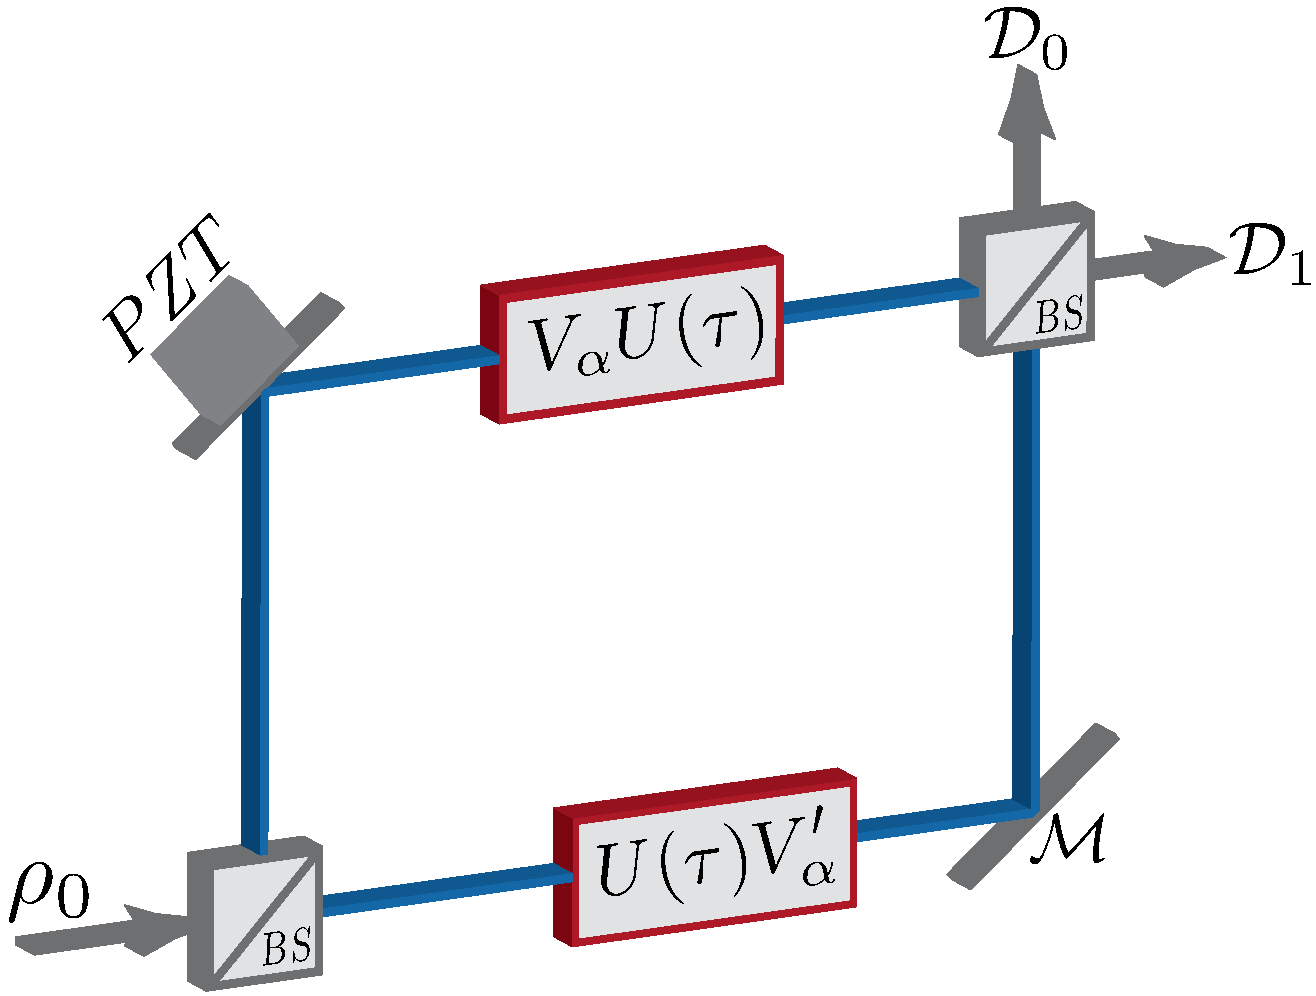
\includegraphics[width=0.45\linewidth]{mz-int}\hspace{1cm}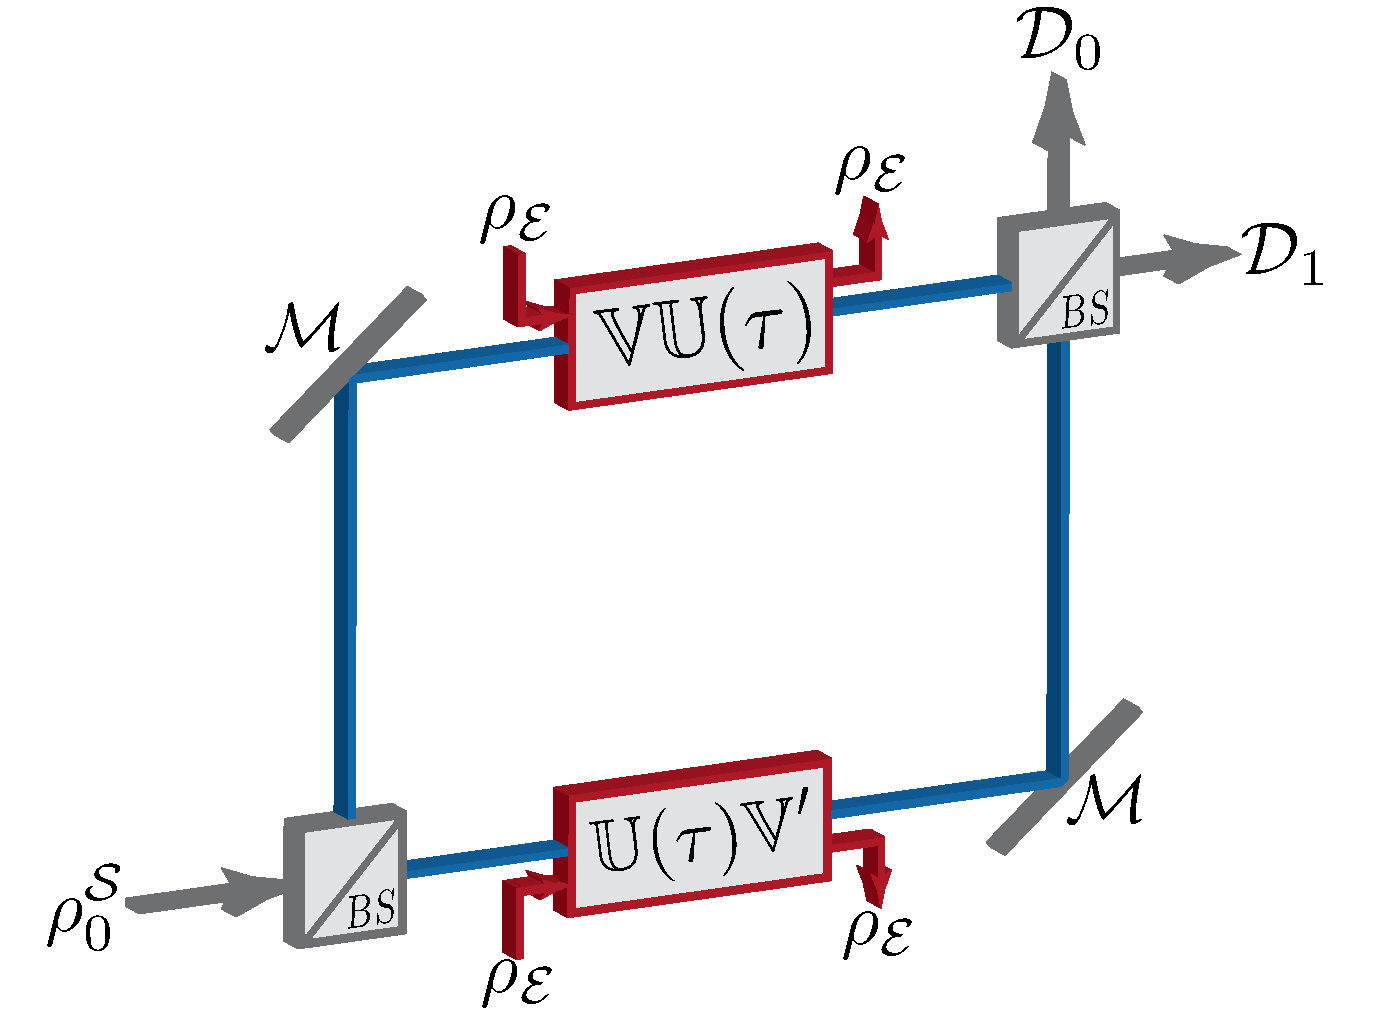
\includegraphics[width=0.45\linewidth]{mz-int-open}
\captionof{figure}{Protocol to measure the characteristic function. Left: In the optical interferometer the input state is split. In the upper path it is imaged by a lens the device that realizes the free evolution $V_{\alpha}$. After this, the process denoted by $U(\tau)$ is implemented and another lens images the final transverse distribution onto the output. In the lower path a similar scheme is realized, but it first goes through the process and then to the free evolution $V_{\alpha}'$ according to the new Hamiltonian. $\mathcal{M}$ is a mirror, $\mathcal{D}_{0}$ and $\mathcal{D}_{1}$ are bulk detectors, and PZT is used to control the phase difference and to alternate between the real and the imaginary parts of the characteristic function. Right: Same as before, but now the process is an open one, realized by means of the interaction of the system with some environment $\mathcal{E}$.} 
\label{fig:set-up}
\end{center}\vspace{1cm}

Assuming that we have a 50:50 beam splitters at the input and output, denoting by $A$ the total intensity in each arm of the interferometer, and summing up over the incoherent contributions of all modes composing the initial thermal state, the light intensity at the output is proportional to
\begin{eqnarray}
I \propto 2A + Re \biggr\{  \sum_{m,n}p_{n}^{I}  |c_{m,n}|^2 \, \mbox{e}^{i(\varepsilon_{m}^{F}-\varepsilon_{n}^{I})s}\biggr\},
\label{c5}
\end{eqnarray}

Comparing this result with the characteristic function (the Fourier transform of Eq. (\ref{eq:work})) we can see that the intensity $I$ is proportional to its real part $I \propto 2A + \mbox{Re}\left[G(s)\right]$, apart from the constant factor $2A$. In this calculation, we considered that the overall phase difference between upper and lower paths was zero. However, the phase difference can be controlled using the PZT shown in Fig. \ref{fig:set-up}, so that we can set it to $\pi/2$ in order to measure the imaginary part of characteristic function. 

%%%%%%%%%%%%%%%%%%%%%%%%%%%%%%%%%%%%%%%%%%%%%%%%%
%%%%%%%%%%%%%%%%%%%%%%%%%%%%%%%%%%%%%%%%%%%%%%%%%
\section*{Example}

We choose a particular process which displaces the linear momentum of the oscillator by $p_{0}$. In this case, the initial and final Hamiltonians in the Schr\"{o}dinger picture, are given by
\begin{equation}
\mathbf{H}_{I} = \frac{\mathbf{P}^{2}}{2m} + \frac{m\omega^{2}}{2}\mathbf{X}^{2}, \hspace{1cm} \mbox{and} \hspace{1cm}  \mathbf{H}_{F} = \frac{\left( \mathbf{P} + p_{0} \right)^{2}}{2m} + \frac{m\omega^{2}}{2}\mathbf{X}^{2},
\label{hamil}
\end{equation}
As they are connected by a similarity transformation $\mathbf{H}_{F} = D^{\dagger}(p_{0}) \mathbf{H}_{I}D(p_{0})$, $D(p_{0}) \equiv e^{-ip_{0}\mathbf{X}/\hbar}$, they have the same energy spectra $\varepsilon^{F}_{n} =\varepsilon^{I}_{n} \equiv \varepsilon_{n} = \hbar\omega\left(n + \frac{1}{2}\right)$ ($n = 0, 1, 2, ...$). The evolution between such Hamiltonians is made by a sudden quench. Considering this process we can compute the characteristic function as
\begin{equation}
G\left(s\right) = \sum_{m,n}\frac{p_{n}^{I}q_{0}^{2(m+n)}e^{-q_{0}^{2}/2}}{2^{m+n}n!m!}e^{is(m - n)}\left\vert\sum_{r=0}^{\min(m,n)}r!2^{r}\binom{m}{r}\binom{n}{r}(-iq_{0})^{-2r}\right\vert^{2},
\label{eq:char_f}
\end{equation}
where $\zeta = \mathcal{W}/\hbar\omega$ is a dimensionless quantity measuring work in units of $\hbar\omega$, while $q_{0}=p_{0}/\sqrt{m\omega\hbar}$ is a dimensionless scale for the quench. $m$ and $\omega$ characterize the oscillator.

Fig. \ref{fig:plots} shows the behavior of the characteristic function for some values of $q_0$ and for some temperatures of the initial thermal state expressed in terms of the ratio $\hbar\omega/kT$.
\begin{center}\vspace{1cm}
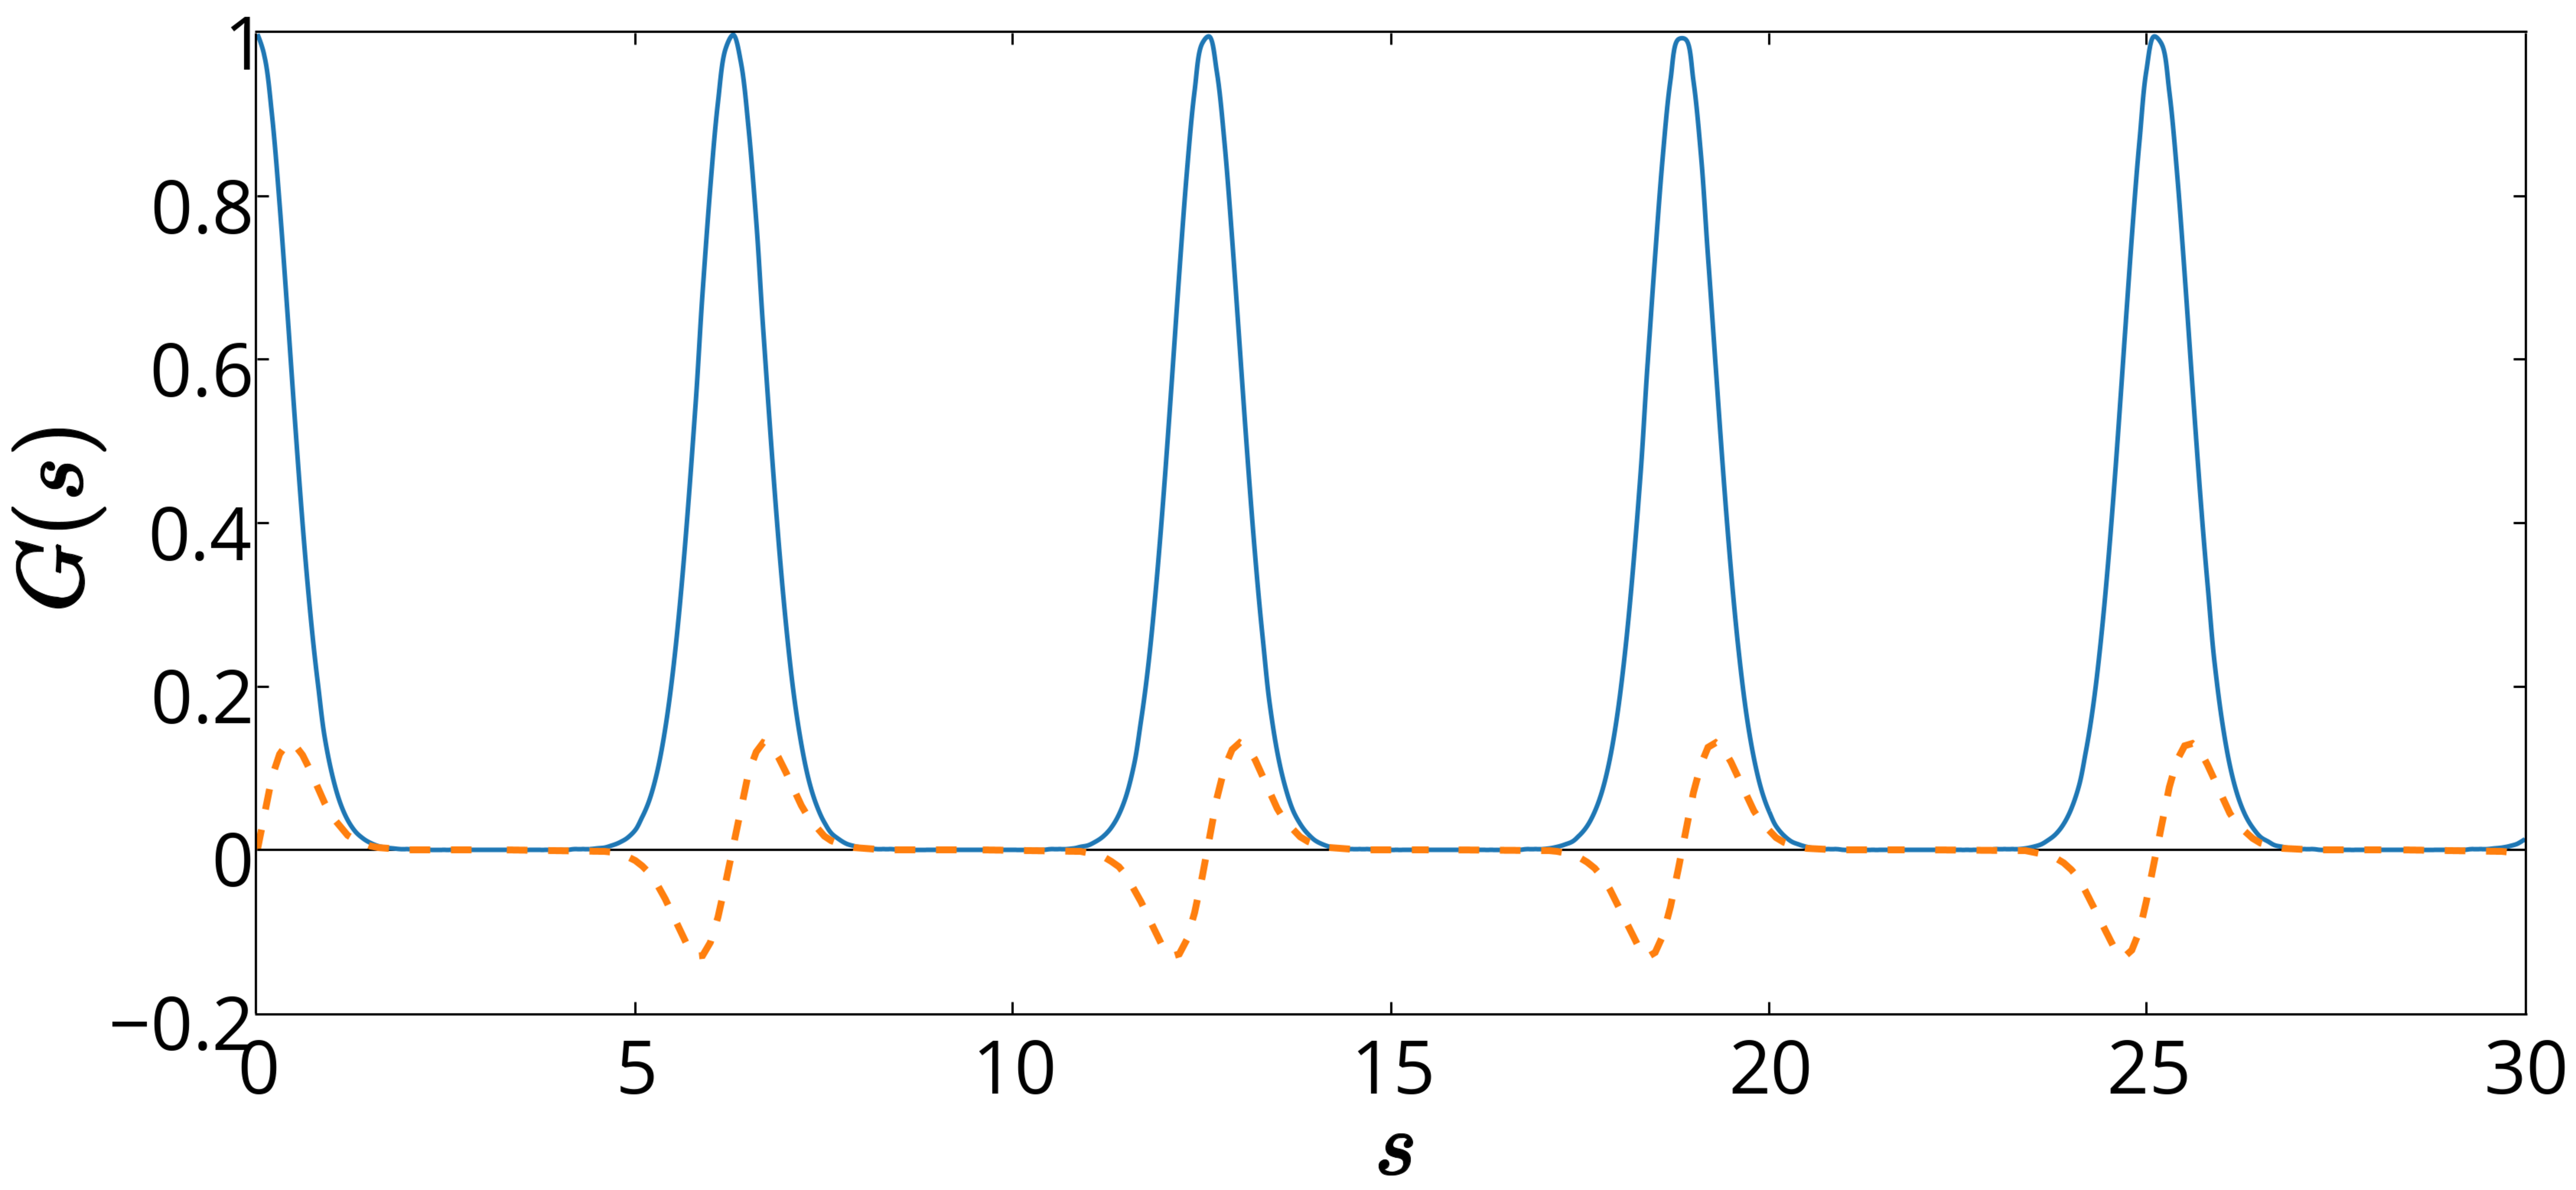
\includegraphics[width=0.45\linewidth]{Char_01}\hspace{1cm}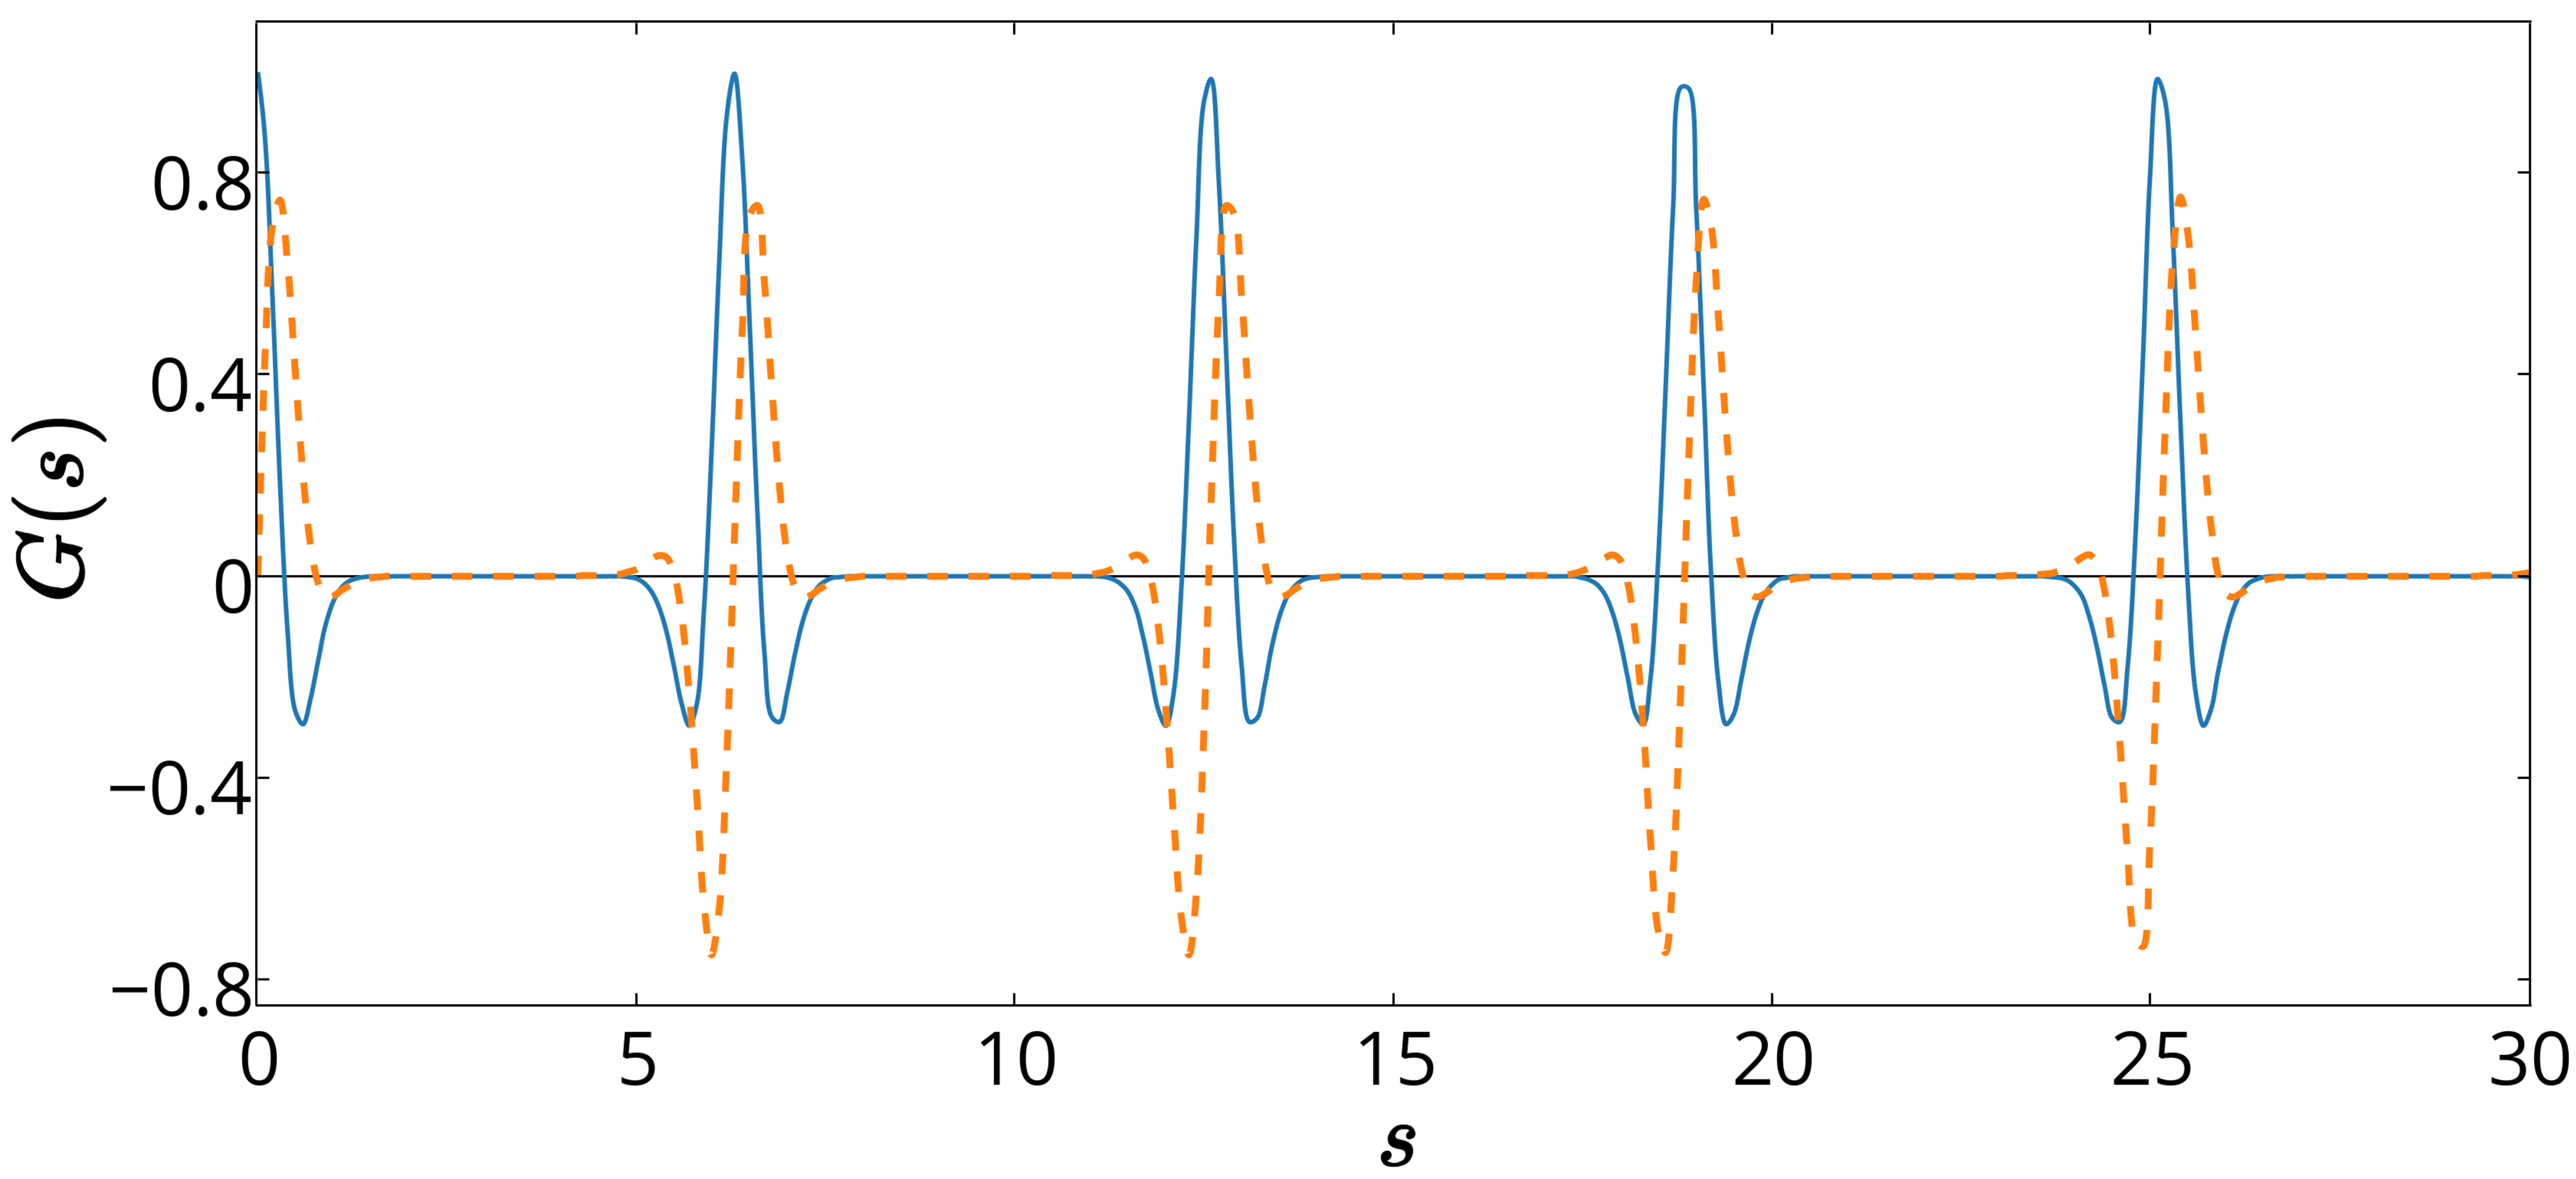
\includegraphics[width=0.45\linewidth]{Char_03}
\captionof{figure}{Characteristic function for the kicked harmonic oscillator. The parameters are $q_0 = 1$ and $\hbar\omega/kT = 0.1$ in the left figure and $q_0 = 3$ and $\hbar\omega/kT = 1$ for the right one. The solid and dashed lines are the real and imaginary parts of the characteristic function, respectively.} 
\label{fig:plots}
\end{center}\vspace{1cm}

%%%%%%%%%%%%%%%%%%%%%%%%%%%%%%%%%%%%%%%%%%%%%%%%%
%%%%%%%%%%%%%%%%%%%%%%%%%%%%%%%%%%%%%%%%%%%%%%%%%
\section*{Discussions}

The proposed experiment is rather simple and allows a high degree of control over the parameters of the system and process. Here are some physical aspects of the set-up that demonstrates its generality and usefulness for the study of thermodynamics of quantum systems.

{\em Versatility of the set-up.} Our scheme relies on the isomorphism between the non-relativistic quantum dynamics of a particle under the action of a given potential and the paraxial Helmholtz equation for the light propagating in a medium with modulated index of refraction. Therefore, by suitably changing the index of refraction we can modify the effective potential of the analogue quantum system.

{\em Open dynamics.} As fluctuation relations still hold for the open dynamic case, we can address questions like how entropy is produced in the system of interest or what are the role played by correlations in thermodynamic processes. Moreover, non-Markovian evolutions can also be addressed.

{\em Quantum versus classical.} We could go from the quantum to the classical regime by increasing the temperature of the initial state. In this case the ratio $\hbar\omega/kT \rightarrow 0$, meaning that the separation between the energy levels would be very small compared to the thermal energy, and the work distribution would tend to a continuous distribution.

%----------------------------------------------------------------------------------------
%	REFERENCES
%----------------------------------------------------------------------------------------
\bibliographystyle{plain} % Plain referencing style
\bibliography{refs} % Use the bibliography file refs.bib

%----------------------------------------------------------------------------------------
%	AFFILIATIONS
%----------------------------------------------------------------------------------------
\section*{Affiliations (publication time)}
$^{1}$Departamento de F\' \i sica, Universidade Federal de Santa Catarina. \\
$^{2}$Universidade Tecnol\'ogica Federal do Paran\'a, Campus Toledo. \\
$^{3}$Instituto Federal de Santa Catarina, Campus Florian\'opolis. \\
$^{4}$Instituto de F\'{i}sica, Universidade Federal de Goi\'{a}s.

%----------------------------------------------------------------------------------------
%	ACKNOWLEDGEMENTS
%----------------------------------------------------------------------------------------
\section*{Acknowledgements}
This work was funded by the Brazilian funding agencies CNPq (Grants No. 401230/2014-7, 445516/2014-3 and 305086/2013-8), CAPES, and the National Institute for Quantum Information (INCT-IQ).

\end{multicols}
\end{document}